\documentclass[11pt,a4paper]{article}
\usepackage[utf8]{inputenc}
\usepackage[T1]{fontenc}
\usepackage[italian]{babel}
\usepackage{lmodern,microtype}
\usepackage[margin=2cm]{geometry}
\usepackage{enumitem}
\usepackage{graphicx,booktabs,float}
\usepackage[hidelinks]{hyperref}
\setlength{\parindent}{0pt}
\setlength{\parskip}{4pt}
\setlist[itemize]{nosep,leftmargin=1.4em,topsep=3pt}
\newcommand{\completare}[1]{\textit{[Da completare: #1]}}
\begin{document}
\begin{center}
{\Large\bfseries Piano degli esperimenti: simulazione e prove sul robot reale}
\end{center}

\textbf{Missione vs esecuzione}

Una missione è una scena con un punto di partenza e un goal assegnato. Un'esecuzione è una singola prova della missione. La stessa missione può quindi essere eseguita più volte.

\textbf{Scopo generale}

L'obiettivo è verificare se Spot, usando una policy che combina immagini e stato del robot, riesce a raggiungere il goal minimizzando il consumo energetico. Considero insieme raggiungimento del goal, consumo energetico, tempo, distanza e cadute. In tutti gli esperimenti, sia simulati sia reali, con \textbf{costo energetico} intendo il \textbf{lavoro meccanico assoluto ai giunti}.

Uso Spot con una camera RGB-D: una ZED X in simulazione e una ZED 2 nelle prove reali. Gli esperimenti sono divisi in simulazione e realtà; per il reale considero le prove indoor in laboratorio. Le eventuali prove outdoor restano da definire.

\section{Esperimenti in simulazione}

\subsection{Primo esempio: scelta fra due percorsi}

Il primo caso è un esempio breve per mostrare in modo semplice il funzionamento del'algoritmo.
Le altre prove più complesse sono fatte in seguito.

Ho allenato una policy con PPO su due disposizioni speculari della stessa scena: un ramo asfaltato, uno roccioso e una zona centrale scivolosa (che simula una lastra di ghiaccio).
L'obiettivo è mostrare la scelta fra due alternative, raggiungendo il goal senza cadere.

\begin{itemize}
\item \textbf{Prove:} 10 esecuzioni, cinque per ciascuna disposizione.
\item \textbf{Start e goal:} partenza nominale a (0, 0) m e arrivo a (4, 4) m, con piccole variazioni iniziali della posizione.
\item \textbf{Cosa mostro:} andamento del training, traiettorie sulle due mappe, raggiungimenti del goal e costo di ogni esecuzione.

\end{itemize}

\subsection{Primo esempio con SAC e sette terreni}

Da questo esperimento in poi, e per tutti quelli successivi, come algoritmo ho usato SAC, che include un incentivo all'esplorazione.
Considero sette terreni con geometrie, attriti e texture scelti per rappresentare superfici reali.

Prima della valutazione più ampia mostro un breve esempio con partenza e goal assegnati, riportando i tragitti di 19 esecuzioni.
Serve a osservare come si comporta la policy in alcuni casi specifici.
Qui mostro il confronto energetico di vari percorsi possibili.

(mi riferisco a quell'esempio che ti avevo mostrato allenato con start e goal fissi, da cui avevo ricavato i due grafici che erano molto interessanti.)


\subsection{Valutazione sulla mappa 7 x 7}

La scena principale è una mappa di 49 celle, ciascuna di 6~m per 3~m, con sette tipi di terreno distribuiti casualmente e presenti in sette celle ciascuno.
La policy è stata allenata con SAC usando punti di partenza e arrivo casuali. La mappa è rimasta fissa durante l'addestramento, per limitarne il carico computazionale, e viene mantenuta uguale anche negli esperimenti: a variare sono i punti di partenza e i goal.

L'obiettivo è osservare il comportamento di Spot quando gli vengono assegnati goal su terreni diversi e a distanze diverse dalla partenza. Verifico se li raggiunge entro il tempo previsto, registrando eventuali timeout o cadute. Osservo inoltre se le scelte di percorso tengono conto del costo del movimento.


\textbf{Prevedo 30 missioni diverse, con un'esecuzione per missione:}
\begin{itemize}
\item 10 con start e goal vicini, a circa 3--6 m;
\item 10 a distanza intermedia, circa 6--12 m;
\item 10 a distanza maggiore, circa 12--18 m.
\end{itemize}

(qui non sono sicurissima di fare 10 10 e 10, e forse ha più senso farne di più nei percorsi lunghi. devo valutare.)

Scelgo \textbf{casualmente} tutte le coppie all'interno di queste fasce, includendo:
\begin{itemize}
\item tragitto semplice su terreno regolare;
\item ghiaccio sul percorso diretto, con spazio per aggirarlo;
\item scale sul percorso diretto, con un passaggio alternativo;
\item scelta fra due percorsi su superfici con costi diversi;
\item più cambi di terreno o più scelte successive.
\end{itemize}

Per queste prove scelgo start e goal fuori da ghiaccio e scale, lasciando però che tali terreni possano trovarsi lungo il tragitto.
Le casistiche possono sovrapporsi: una missione può includere una deviazione e più cambi di superficie.

Mostro una panoramica delle 30 traiettorie, confrontandole con il percorso rettilineo e confrontandone i costi.
Faccio quindi un riepilogo di energia consumata (magari mostrando il guadagno rispetto al non utilizzo della policy), tempo impiegato, fallimenti e eventuali cadute.

\section{Esperimenti sul robot reale}

\subsection{Indoor: pavimento grigio vs telo verde}

Per le prove in laboratorio semplifico la scena a due superfici: un terreno grigio (che simula il pavimento del laboratorio) e un terreno verde (che simula un telo/cartoncino verde disposto sul pavimento in alcune aree).
In simulazione il grigio consente il movimento ordinario; sul verde è applicata una maggiore resistenza al moto, per rendere l'attraversamento più faticoso e costoso anche dal punto di vista temporale.
Nella realtà il terreno verde non ha le stesse caratteristiche fisiche della simulazione, ma serve a rappresentare visivamente la superficie e a distinguerla dal pavimento grigio.

Lo scopo è verificare se il comportamento appreso in simulazione si trasferisce alla stanza reale: Spot dovrebbe valutare quando è conveniente attraversare la zona verde e quando invece conviene deviare, e di quanto.

\textbf{Prima della prova reale prevedo 10 missioni simulate} in cui start e goal sono scelti \textbf{randomicamente} (a una distnaza che va dai 2 m ai 10 m), considerando le seguenti fasce:

\begin{itemize}
\item tragitti sul solo grigio;
\item una zona verde davanti al robot e una deviazione disponibile;
\item più zone verdi lungo il tragitto;
\item zona verde a destra o a sinistra, per variare il lato della deviazione;
\item goal sul verde, per verificare che la superficie venga attraversata quando serve.
\end{itemize}


\textbf{Nel laboratorio propongo cinque missioni, ciascuna ripetuta due volte: 10 esecuzioni.}
\begin{itemize}
\item un tragitto sul grigio;
\item due tragitti con una zona verde sul percorso diretto;
\item un tragitto con più zone verdi da evitare (deviando leggermente);
\item un tragitto con goal sulla zona verde.
\end{itemize}

Le coordinate saranno scelte in base allo spazio della stanza e poi mantenute uguali nelle due ripetizioni.

Mostro la scena reale, i percorsi seguiti e il confronto fra raggiungimento del goal, energia e tempo utilizando la policy e senza utilizzarla. 

(poi qui in base ai tempi e alla fattibilità valutiamo se estendere gli esperimenti con altre ripetizioni o altre nuove missioni)

\subsection{Indoor: pavimento grigio vs zona nera}

La seconda scena ha la stessa impostazione, ma il verde viene sostituito dal nero.
In simulazione il nero rappresenta una superficie scivolosa con le stesse proprietà fisiche del ghiaccio, sulla quale Spot perde l'equilibrio e cade molto facilmente.
Lo scopo è verificare se la policy impara a evitarla e mantiene questo comportamento nel laboratorio.

\textbf{Prevedo 10 missioni simulate}, sempre ad una distanza che varia dai 2 m ai 10 m, con start e goal scelti randomicamente all'interno di varie fasce: tragitti senza nero, una zona nera sul percorso diretto, più zone nere e passaggi alternativi su lati diversi.
In questo caso escludo casistiche in cui il goal si trova sul terreno nero, in quanto sarebbe non raggiungibile dal robot.

\textbf{Sul reale propongo cinque missioni ripetute due volte: 10 esecuzioni.}
\begin{itemize}
\item un tragitto sul grigio;
\item due tragitti con una zona nera davanti al robot, variando il lato del passaggio libero;
\item un tragitto con più zone nere;
\item un tragitto più lungo con scelte successive.
\end{itemize}

(anche qui in base alle tempistiche valuto ulteriori esperimenti)

Nel laboratorio delimito le zone con cartelloni neri.
Questi rappresentano visivamente la superficie da evitare, ma non riproducono necessariamente l'attrito del ghiaccio. La prova reale verifica quindi soprattutto se Spot evita la regione associata al terreno scivoloso in simulazione. Mostro traiettorie, goal raggiunti, eventuali attraversamenti del nero e altri esiti.

\subsection{Outdoor}

Le prove all'aperto sono un'estensione possibile. Per ora non ne definisco il protocollo; la scena e l'eventuale training su asfalto, erba e una terza superficie verranno valutati in seguito.

\section{Dati da salvare e risultati da mostrare}

Per ogni esecuzione salvo:
\begin{itemize}
\item scena, modello utilizzato, posizione dello start e del goal;
\item distanza in linea retta fra start e goal;
\item traiettoria e distanza effettivamente percorsa;
\item lavoro meccanico assoluto ai giunti dell'intera missione;
\item tempo fino al raggiungimento del goal o all'interruzione;
\item esito: successo, caduta, timeout, uscita dall'area o arresto dell'operatore;
\end{itemize}

Il tempo e il costo energetico includono l'eventuale allineamento iniziale, che fanno parte dell'esecuzione.


\clearpage
\section{Risultati degli esperimenti}
\label{sec:risultati-esperimenti}

In questa parte raccolgo, nello stesso ordine del protocollo, i risultati degli esperimenti effettivamente eseguiti. Per ogni caso riporto le missioni assegnate, le traiettorie e i dati registrati. Le prove ancora da valutare o da svolgere sono indicate separatamente.

\subsection{Risultati del caso 1.1: scelta fra due percorsi}
\label{sec:risultati-caso-1-1}

Questi risultati si riferiscono all'esempio descritto nella sezione 1.1. Ho usato la policy di navigazione allenata con PPO nel caso \texttt{multi\_terrain\_test13}, prendendo il modello finale dopo 100.000 transizioni complessive distribuite su 32 ambienti paralleli. DINOv2 e il controllore locomotorio erano già preaddestrati.

Ho assegnato dieci missioni, ciascuna eseguita una volta: cinque sulla mappa A, con le rocce a destra e l'asfalto a sinistra, e cinque sulla mappa B, con la disposizione speculare. Ogni mappa contiene nove celle di $2\times2$~m; la cella centrale rappresenta il ghiaccio.

\subsubsection{Scelta delle coordinate}

Sono partita dallo start nominale $(0,0)$~m e dal goal nominale $(4,4)$~m. A ciascuna delle quattro coordinate, due dello start e due del goal, ho aggiunto una perturbazione casuale indipendente, estratta da una distribuzione uniforme tra $-0{,}05$~m e $+0{,}05$~m. Il rumore ha quindi media nulla e deviazione standard di circa $0{,}029$~m per coordinata. Il limite di 5~cm si applica separatamente a $x$ e a $y$.

Le coordinate sono state estratte una sola volta e poi mantenute fisse per tutta la rispettiva esecuzione, senza aggiungere altro rumore durante il movimento. L'orientamento iniziale è rimasto pari a $45^\circ$, come nel training. La tabella~\ref{tab:coordinate-caso-1-1} riporta le dieci missioni.

\begin{table}[H]
\centering
\caption{Coordinate assegnate alle dieci missioni del caso 1.1. Le coordinate sono espresse nel riferimento della mappa.}
\label{tab:coordinate-caso-1-1}
\begingroup
\small
\setlength{\tabcolsep}{9pt}
\renewcommand{\arraystretch}{1.15}
\begin{tabular}{ccrrrr}
\toprule
Mappa & Episodio & Start $x$ [m] & Start $y$ [m] & Goal $x$ [m] & Goal $y$ [m] \\
\midrule
A & 1 & $-0{,}0289$ & $0{,}0005$ & $3{,}9883$ & $4{,}0234$ \\
A & 2 & $-0{,}0250$ & $0{,}0104$ & $3{,}9616$ & $4{,}0260$ \\
A & 3 & $-0{,}0065$ & $-0{,}0324$ & $3{,}9974$ & $3{,}9708$ \\
A & 4 & $-0{,}0269$ & $-0{,}0069$ & $3{,}9525$ & $3{,}9805$ \\
A & 5 & $-0{,}0408$ & $0{,}0188$ & $4{,}0362$ & $4{,}0170$ \\
\midrule
B & 1 & $-0{,}0159$ & $0{,}0339$ & $4{,}0441$ & $3{,}9516$ \\
B & 2 & $0{,}0123$ & $-0{,}0173$ & $4{,}0349$ & $3{,}9913$ \\
B & 3 & $-0{,}0204$ & $-0{,}0445$ & $4{,}0249$ & $4{,}0129$ \\
B & 4 & $0{,}0158$ & $-0{,}0329$ & $3{,}9567$ & $4{,}0159$ \\
B & 5 & $0{,}0060$ & $0{,}0283$ & $3{,}9837$ & $3{,}9914$ \\
\bottomrule
\end{tabular}
\endgroup
\end{table}

\subsubsection{Traiettorie e dati delle esecuzioni}

La figura~\ref{fig:traiettorie-caso-1-1} mostra le cinque traiettorie registrate su ciascuna mappa. Lo stesso numero di episodio è usato nei grafici e nelle tabelle della rispettiva mappa. I punti indicano le partenze, le stelle i goal e le croci le posizioni finali. Il cerchio tratteggiato indica il raggio di arrivo di $0{,}55$~m: la missione termina quando Spot entra in questa zona senza cadere o uscire dalla mappa. Il limite di tempo è di 40~s.

\begin{figure}[H]
\centering
\begin{minipage}[t]{0.49\textwidth}
\centering
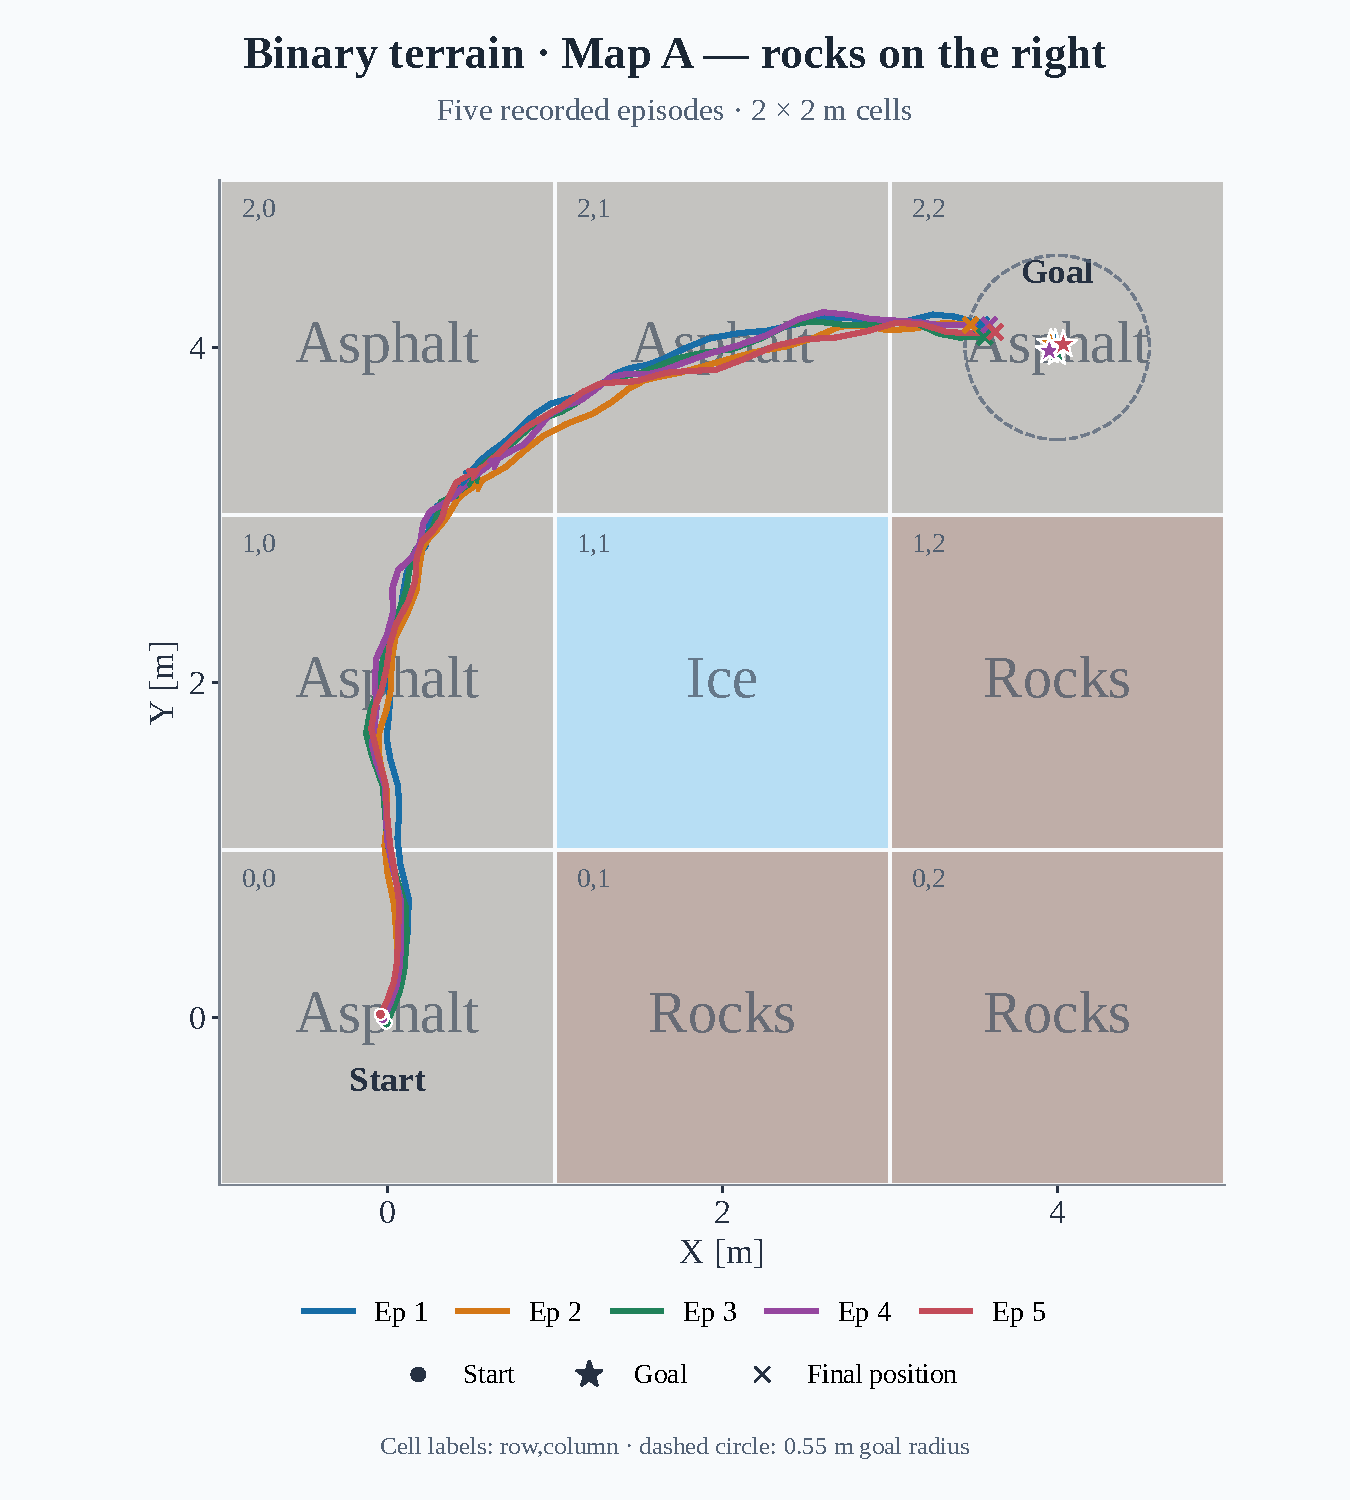
\includegraphics[width=\linewidth]{figure/map_a_routes.pdf}
\end{minipage}\hfill
\begin{minipage}[t]{0.49\textwidth}
\centering
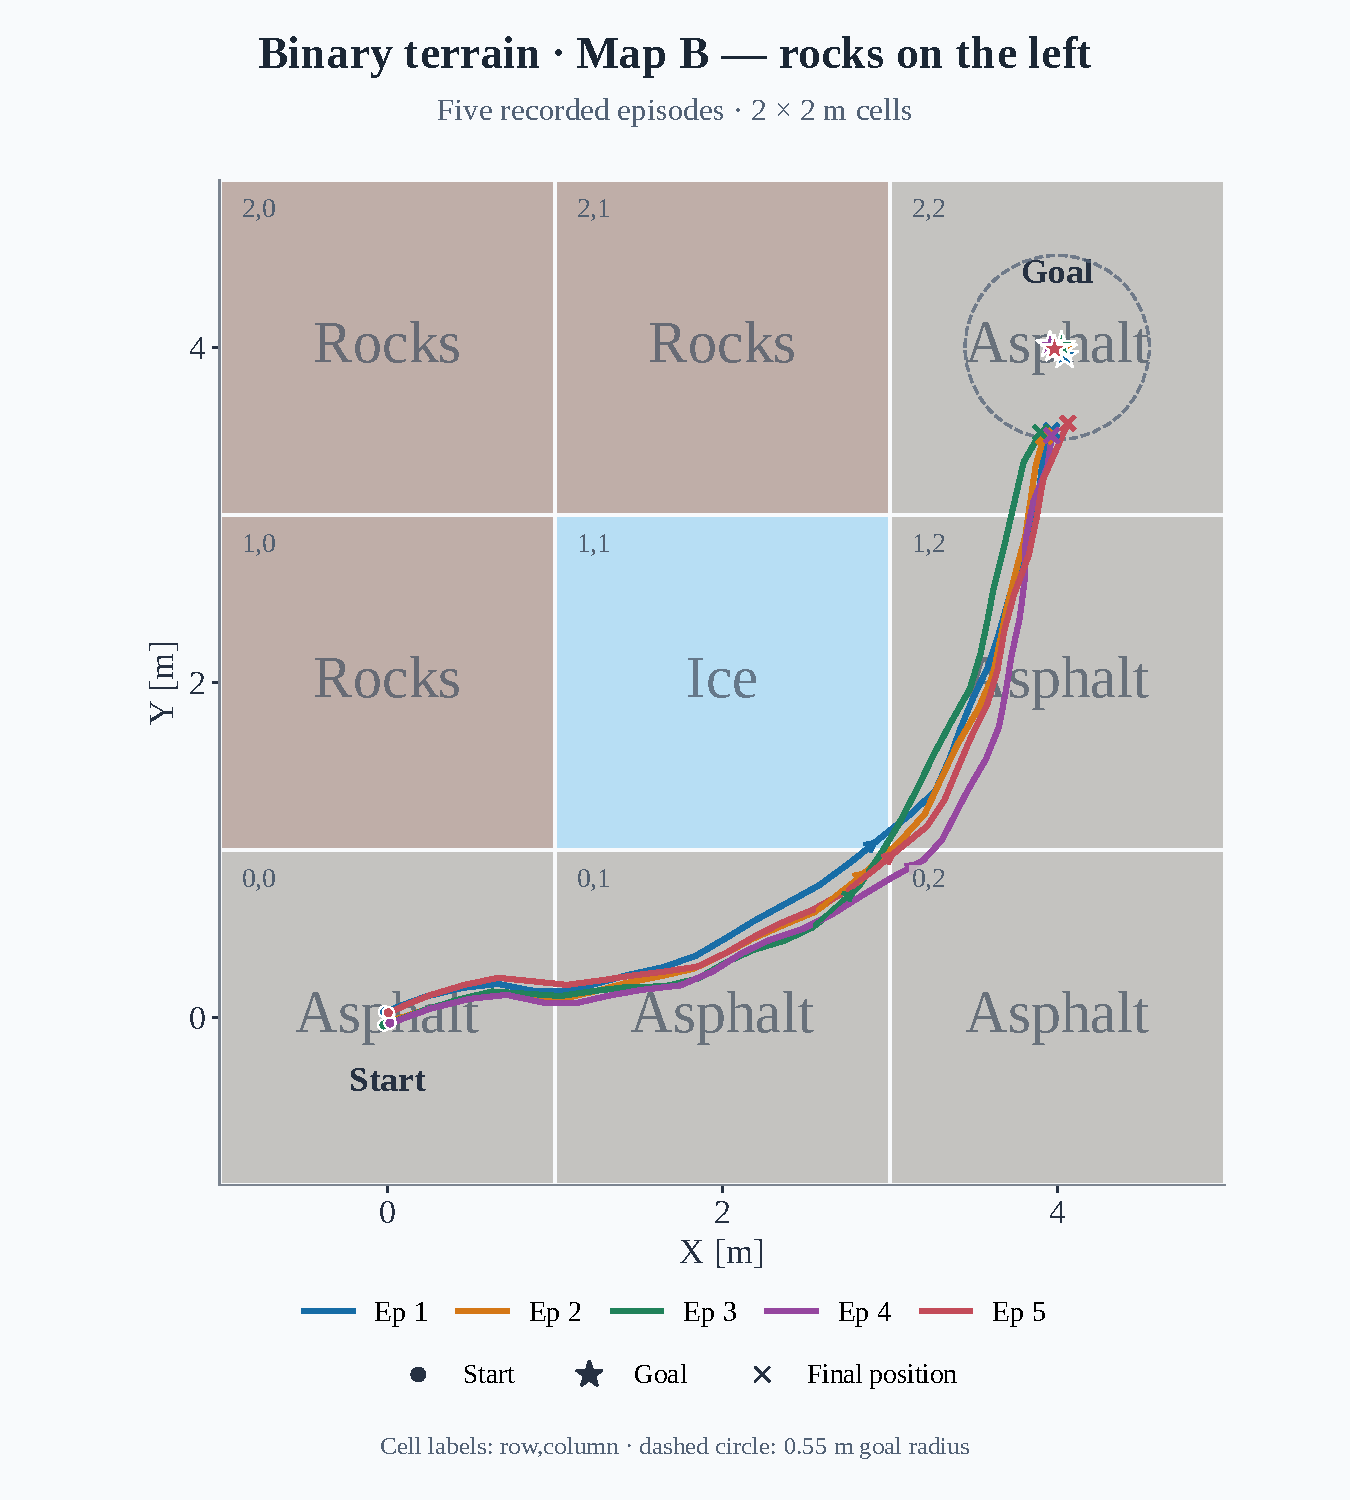
\includegraphics[width=\linewidth]{figure/map_b_routes.pdf}
\end{minipage}
\caption{Traiettorie del caso 1.1: mappa A a sinistra e mappa B a destra. Ogni colore identifica un episodio; gli indici nelle celle indicano riga e colonna, a partire da zero. Gli assi sono espressi in metri.}
\label{fig:traiettorie-caso-1-1}
\end{figure}

Le tabelle~\ref{tab:exp1-1-map-a} e~\ref{tab:exp1-1-map-b} riportano distanza effettivamente percorsa, lavoro meccanico assoluto ai giunti, tempo ed esito. Il tempo è quello simulato e il costo energetico comprende l'intera missione, dalla partenza alla sua conclusione. Le coordinate sono ripetute nelle due tabelle per rendere ogni risultato leggibile anche separatamente.

% Recorded results only. Requires booktabs in the thesis preamble.
% Insert with \input{path/to/tabels_exp1_1.tex}.
% Coordinates: (x; y) on one line.
\begin{table}[H]
\centering
\caption{Risultati dei cinque episodi sulla mappa A, con le rocce a destra.}
\label{tab:exp1-1-map-a}
\begingroup
\fontsize{9.5}{11.5}\selectfont
\setlength{\tabcolsep}{2.5pt}
\renewcommand{\arraystretch}{1.25}
\begin{tabular}{@{}c cc cccc c@{}}
\toprule
\shortstack{Ep.} &
\shortstack{Start $(x;y)$\\{}[m]} &
\shortstack{Goal $(x;y)$\\{}[m]} &
\shortstack{Distanza\\percorsa [m]} &
\shortstack{Energia\\{}[J]} &
\shortstack{Tempo\\{}[s]} &
\shortstack{Velocità\\media [m/s]} &
\shortstack{Esito} \\
\midrule
1 & $(-0{,}0289;\,0{,}0005)$ & $(3{,}9883;\,4{,}0234)$ & $6{,}23$ & $1049{,}0$ & $7{,}2$ & $0{,}87$ & Successo \\
2 & $(-0{,}0250;\,0{,}0104)$ & $(3{,}9616;\,4{,}0260)$ & $6{,}17$ & $1011{,}4$ & $6{,}9$ & $0{,}89$ & Successo \\
3 & $(-0{,}0065;\,-0{,}0324)$ & $(3{,}9974;\,3{,}9708)$ & $6{,}31$ & $1054{,}3$ & $7{,}1$ & $0{,}89$ & Successo \\
4 & $(-0{,}0269;\,-0{,}0069)$ & $(3{,}9525;\,3{,}9805)$ & $6{,}28$ & $1069{,}1$ & $7{,}1$ & $0{,}88$ & Successo \\
5 & $(-0{,}0408;\,0{,}0188)$ & $(4{,}0362;\,4{,}0170)$ & $6{,}26$ & $1057{,}9$ & $7{,}0$ & $0{,}89$ & Successo \\
\bottomrule
\end{tabular}
\endgroup
\par\smallskip
\begin{minipage}{\linewidth}
\footnotesize
Gli episodi 1--5 corrispondono alle missioni A1--A5. Le coordinate di Start e Goal sono riportate come $(x;y)$, in metri.
La distanza percorsa indica la lunghezza della traiettoria effettivamente seguita dal robot. La velocità media è il rapporto fra questa distanza e il tempo totale dell'episodio.
L'energia \`e il lavoro meccanico assoluto ai giunti, misurato fino alla conclusione dell'episodio.
Il successo richiede una distanza dal goal non superiore a $0{,}55$~m, senza cadute o uscite dalla mappa; il timeout \`e fissato a $40$~s.
\end{minipage}
\end{table}

\begin{table}[H]
\centering
\caption{Risultati dei cinque episodi sulla mappa B, con le rocce a sinistra.}
\label{tab:exp1-1-map-b}
\begingroup
\fontsize{9.5}{11.5}\selectfont
\setlength{\tabcolsep}{2.5pt}
\renewcommand{\arraystretch}{1.25}
\begin{tabular}{@{}c cc cccc c@{}}
\toprule
\shortstack{Ep.} &
\shortstack{Start $(x;y)$\\{}[m]} &
\shortstack{Goal $(x;y)$\\{}[m]} &
\shortstack{Distanza\\percorsa [m]} &
\shortstack{Energia\\{}[J]} &
\shortstack{Tempo\\{}[s]} &
\shortstack{Velocità\\media [m/s]} &
\shortstack{Esito} \\
\midrule
1 & $(-0{,}0159;\,0{,}0339)$ & $(4{,}0441;\,3{,}9516)$ & $5{,}93$ & $952{,}4$ & $6{,}0$ & $0{,}99$ & Successo \\
2 & $(0{,}0123;\,-0{,}0173)$ & $(4{,}0349;\,3{,}9913)$ & $5{,}93$ & $923{,}2$ & $6{,}0$ & $0{,}99$ & Successo \\
3 & $(-0{,}0204;\,-0{,}0445)$ & $(4{,}0249;\,4{,}0129)$ & $5{,}99$ & $923{,}0$ & $6{,}0$ & $1{,}00$ & Successo \\
4 & $(0{,}0158;\,-0{,}0329)$ & $(3{,}9567;\,4{,}0159)$ & $6{,}11$ & $977{,}9$ & $6{,}2$ & $0{,}98$ & Successo \\
5 & $(0{,}0060;\,0{,}0283)$ & $(3{,}9837;\,3{,}9914)$ & $6{,}07$ & $959{,}0$ & $6{,}2$ & $0{,}98$ & Successo \\
\bottomrule
\end{tabular}
\endgroup
\par\smallskip
\begin{minipage}{\linewidth}
\footnotesize
Gli episodi 1--5 corrispondono alle missioni B1--B5. Le coordinate di Start e Goal sono riportate come $(x;y)$, in metri.
La distanza percorsa indica la lunghezza della traiettoria effettivamente seguita dal robot. La velocità media è il rapporto fra questa distanza e il tempo totale dell'episodio.
L'energia \`e il lavoro meccanico assoluto ai giunti, misurato fino alla conclusione dell'episodio.
Il successo richiede una distanza dal goal non superiore a $0{,}55$~m, senza cadute o uscite dalla mappa; il timeout \`e fissato a $40$~s.
\end{minipage}
\end{table}



In tutte e dieci le esecuzioni Spot ha raggiunto il goal senza cadute o timeout, scegliendo il ramo asfaltato. Nella mappa A la distanza media percorsa è stata di $6{,}76$~m e il tempo medio di $10{,}32$~s; nella mappa B i valori sono stati rispettivamente $6{,}00$~m e $6{,}08$~s. I percorsi non sono quindi perfettamente speculari. Un'eventuale prova dedicata a questa differenza resta da valutare.

\subsubsection{ANCORA DA FARE --- CONFRONTO ENERGETICO DA VALUTARE}

\textbf{Il confronto descritto di seguito non è stato ancora eseguito. Occorre ancora decidere se realizzarlo e definirne la procedura.}

In questo caso il percorso rettilineo fra start e goal attraversa la zona centrale scivolosa. Senza la policy di navigazione che sceglie una deviazione, ci si aspetta che Spot, andando dritto, cada sul ghiaccio. Una prova rettilinea non è stata ancora svolta su queste dieci missioni. Il suo costo energetico includerebbe quindi, nell'eventualità della caduta, un'esecuzione interrotta e non il completamento della stessa missione: per questo non lo considero il confronto energetico principale per questo esempio.

Una possibilità da valutare è confrontare il percorso scelto sull'asfalto con un percorso speculare sul ramo roccioso, di lunghezza corrispondente. L'obiettivo sarebbe osservare quanto lavoro meccanico richiede Spot per percorrere una strada analoga sulle rocce anziché sull'asfalto.

Il costo di questa alternativa deve essere misurato con nuove prove in simulazione e non è ricavabile direttamente dai consumi già registrati sull'asfalto. Restano da definire il modo di seguire il percorso e la velocità di riferimento, valutando se usare la velocità media dei singoli episodi. Andranno mantenuti criteri confrontabili fra le due superfici, registrando anche eventuali cadute o mancati completamenti.



VOLENDO SI POSSONO USARE L STESSE TRAIETTORIE SCAMBIANDO LE MAPPE, COSI SI FINISCE SULL'ALTRO TERRENO.


\textbf{Per ora questa parte resta da fare e da discutere.}

\textbf{ANCORA DA FARE}
\begin{itemize}
\item Rifare uno dei due test: in una delle due mappe Spot passa molto più distante dal ghiaccio rispetto all'altra.
\item Provare ad aumentare il rumore sullo start e sul goal.
\item Confronto con le rocce: come realizzarlo? Definire il percorso da seguire, il controllore e la velocità di riferimento.
\end{itemize}

\clearpage
\subsection{Caso 1.2: esempio punto a punto sulla mappa grande --- DA FARE}
\label{sec:risultati-caso-1-2}

In questo esempio, richiamato nella sezione 1.2 del protocollo, il training è stato svolto su una mappa grande, mantenendo fissi start e goal e senza aggiungere rumore alle loro coordinate. Lo scopo era osservare se, con l'allenamento, Spot imparasse a scegliere un percorso conveniente fra i diversi terreni. Le traiettorie ottenute sono interessanti e saranno descritte più avanti.

\textbf{Questa parte è provvisoria e da rifare.} Per ora riporto i due grafici già disponibili, senza aggiungere un'analisi dei risultati. I grafici provengono da una \textbf{policy allenata in precedenza, più vecchia rispetto a quelle attualmente considerate}; la policy di riferimento e la presentazione finale saranno da aggiornare.

Ho preso i file originali dalla cartella:
\par{\small\path{spot_rl_energy_navigation/medium_distance_choice/results/}\par}
\begin{itemize}
\item \path{medium_eval_20261007_114130_routes_outcomes.svg};
\item \path{medium_eval_20261007_114130_routes_successes.svg}.
\end{itemize}
Le figure seguenti sono conversioni in PDF di questi SVG, mantenuti per ora con il loro aspetto originale. In seguito saranno rifatte con lo stile usato per il caso 1.1.

\begin{figure}[H]
\centering
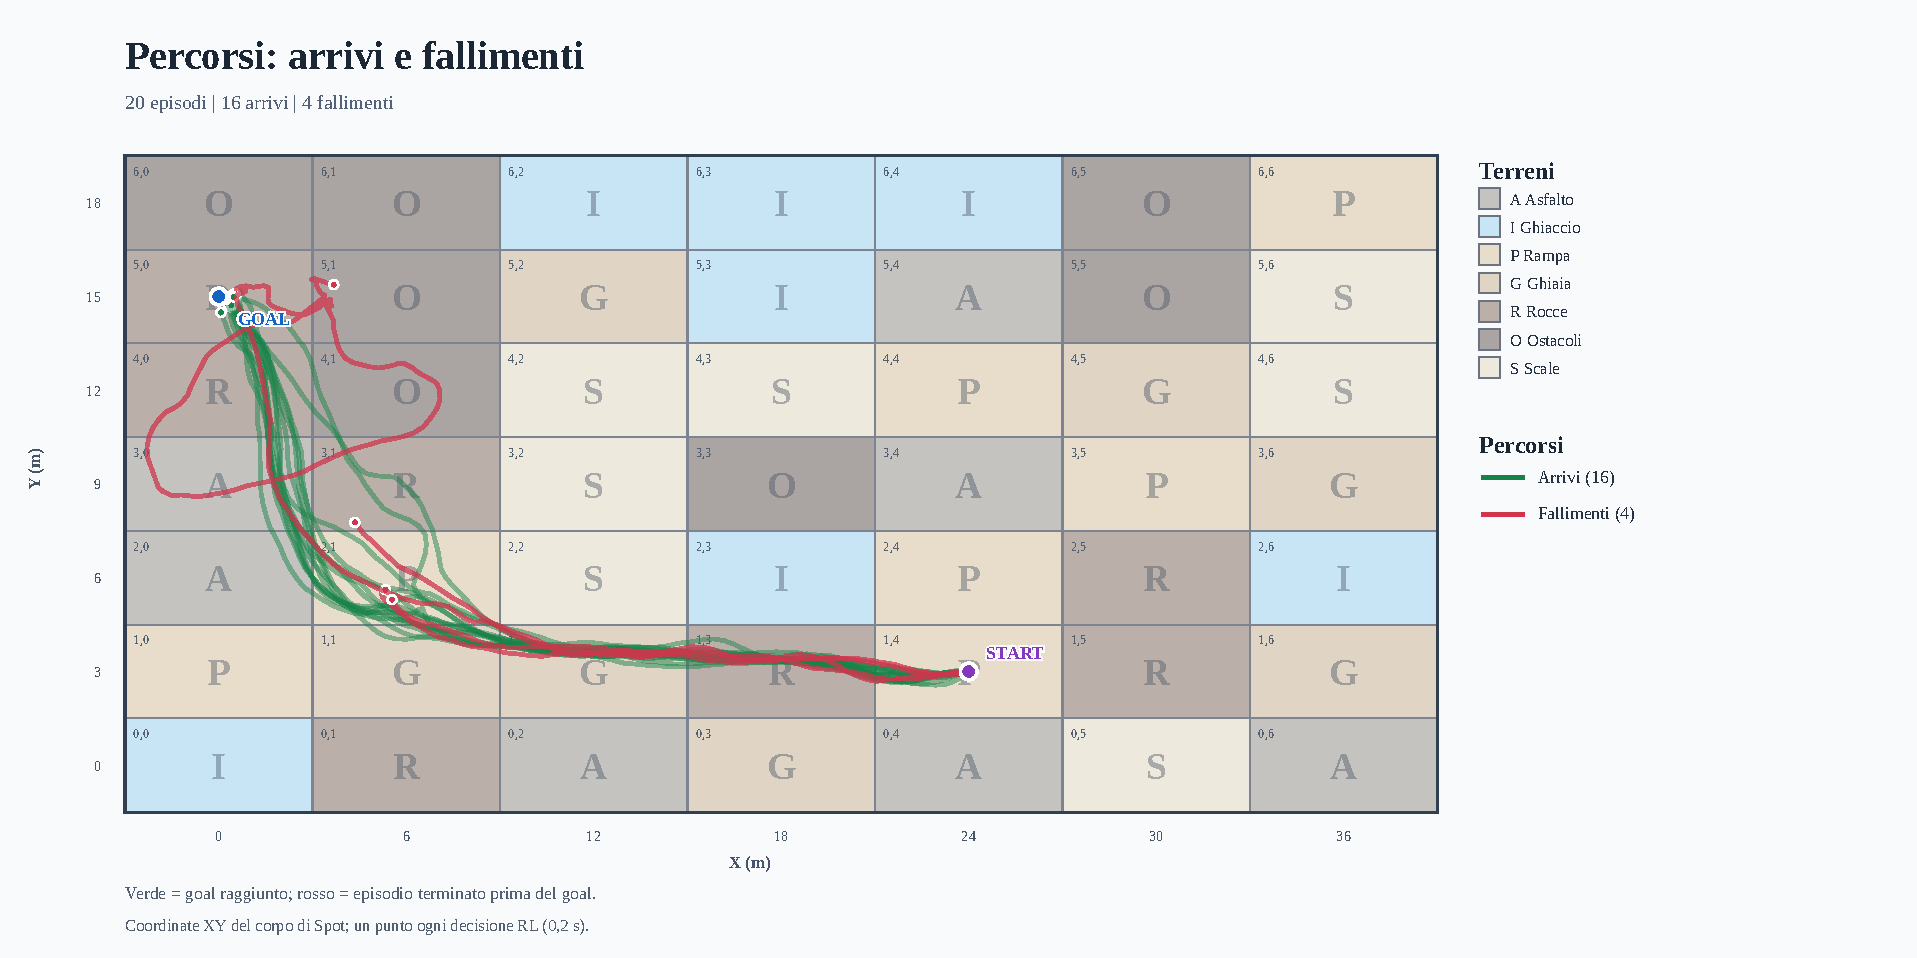
\includegraphics[width=\linewidth]{figure/medium_eval_20261007_114130_routes_outcomes.pdf}
\caption{Grafico provvisorio degli esiti delle esecuzioni: versione precedente della policy. DA RIFARE.}
\label{fig:medium-routes-outcomes-provvisorio}
\end{figure}

\begin{figure}[H]
\centering
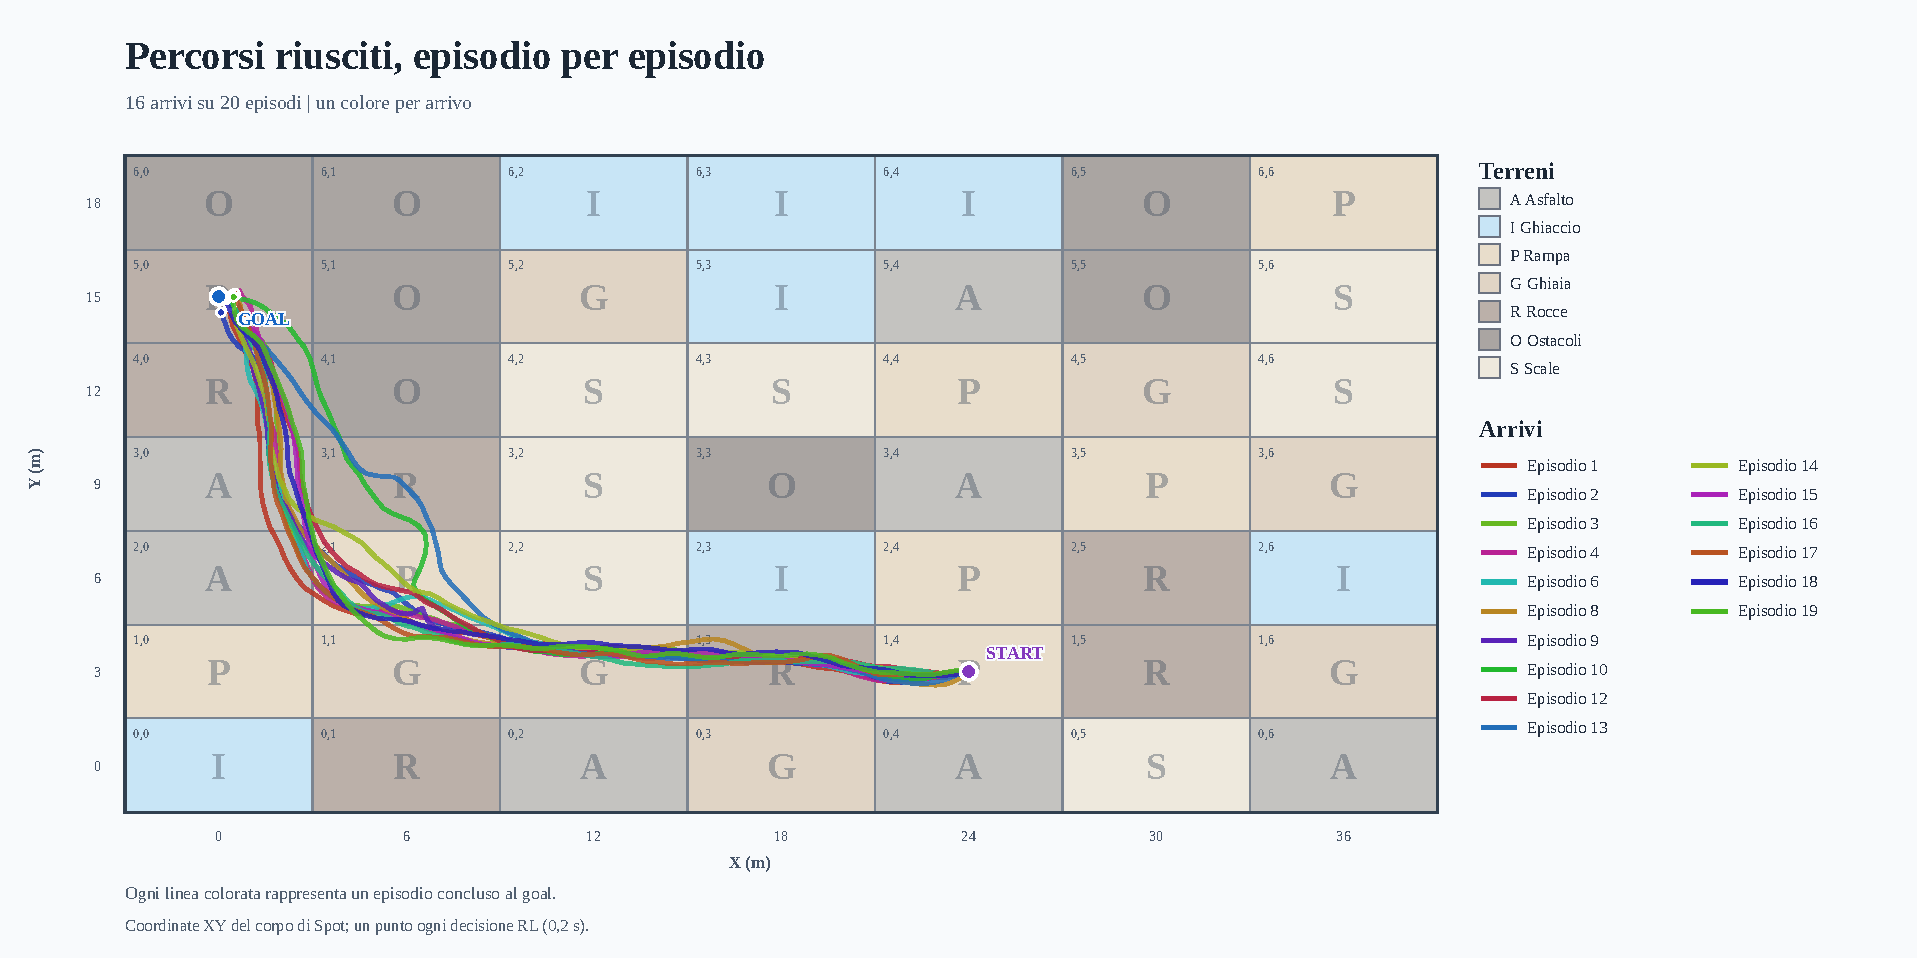
\includegraphics[width=\linewidth]{figure/medium_eval_20261007_114130_routes_successes.pdf}
\caption{Grafico provvisorio delle traiettorie con arrivo al goal: versione precedente della policy. DA RIFARE.}
\label{fig:medium-routes-successes-provvisorio}
\end{figure}

\subsection{Caso 1.3: missioni sulla mappa grande --- DA FARE}
\label{sec:risultati-caso-1-3}

\subsubsection{ANCORA DA FARE --- DISTANZA GEODETICA DA VALUTARE}

Più avanti valuteremo se calcolare anche la distanza geodetica fra start e goal, intesa come la lunghezza del percorso più corto nelle zone considerate percorribili. Per questa stima occorrerà definire le zone da escludere, come ghiaccio e scale, e un margine dai loro bordi che tenga conto dell'ingombro di Spot. Il calcolo non è stato ancora eseguito.

Questa distanza potrebbe aiutare a descrivere quanto una missione richiede di deviare rispetto al segmento diretto. Non misura il consumo energetico e non sostituisce le prove del riferimento rettilineo. Per ora le due distanze previste di 6 e 18~m rimangono distanze in linea retta fra start e goal.

\end{document}
